\documentclass{homework}
\usepackage{enumitem}

\newcommand{\hwclass}{Math 6108}
\newcommand{\hwname}{Jacob Hauck}
\newcommand{\hwtype}{Homework}

\newcommand{\R}{\textbf{R}}
\newcommand{\dee}{\;\text{d}}
\newcommand{\eps}{\varepsilon}
\newcommand{\pl}[2]{\frac{\partial #1}{\partial #2}}
\newcommand{\dl}[2]{\frac{\text{d} #1}{\text{d} #2}}
\newcommand{\sgn}{\text{sgn}}
\newcommand{\bigoh}{\mathcal{O}}

\usepackage{float}
\usepackage{booktabs}
\usepackage{makecell}
\usepackage[ruled,linesnumbered]{algorithm2e}

\renewcommand{\hwtype}{Final Project}
\newcommand{\hwnum}{}
\renewcommand{\questiontype}{Problem}

\begin{document}
	\maketitle
	
	Consider the following second-order ODE with Dirichlet boundary conditions:
	\begin{align}
		\label{eq:ode}
		\dl{}{x}\left(c(x)\dl{u(x)}{x}\right) &= f(x),\qquad a \le x \le b, \\
		\label{eq:bc}
		u(a) = g_a,\quad u(b) &= g_b.
	\end{align}
	
	\question
	Consider the second-order ODE (\ref{eq:ode}). Multiplying by $v \in H^1([a,b])$ and integrating by parts gives
	\begin{equation}
		\label{eq:ibp}
		\int_a^bfv = c(b)u'(b)v(b) - c(a)u'(a)v(a) - \int_a^b cu'v.
	\end{equation}
	
	\begin{alphaparts}
		\questionpart Suppose we have the boundary conditions
		\begin{equation}
			u'(a) = p_a, \qquad u(b) = g_b.
		\end{equation}
		Equation (\ref{eq:ibp}) still holds, and we can impose the condition $v(b) = 0$ because we already know that $u(b) = p_b$. Since $u'(a) = p_a$, equation (\ref{eq:ibp}) becomes
		\begin{equation}
			\int_a^b fv = -c(a)p_av(a) - \int_a^bcu'v'
		\end{equation}
		for all $v \in H^1([a,b])$ such that $v(b) = 0$, which is our weak formulation of (\ref{eq:ode}) with the given boundary conditions.
		
		\questionpart Suppose we have the boundary conditions
		\begin{equation}
			u'(a) = p_a, \qquad u'(b) + q_bu(b) = p_b.
		\end{equation}
		Equation (\ref{eq:ibp}) still holds. Since $u'(b) = p_b - q_bu(b)$, and $u'(a) = p_a$, we get
		\begin{equation}
			\int_a^bfv = c(b)(p_b - q_bu(b))v(b) - c(a)p_av(a) - \int_a^bcu'v'
		\end{equation}
		for all $v \in H^1([a,b])$, which is our weak formulation of (\ref{eq:ode}) with the given boundary conditions.
		
		\questionpart Suppose we have the boundary conditions
		\begin{equation}
 			u'(a) = p_a,\qquad u'(b) = p_b.
		\end{equation}
		Equation (\ref{eq:ibp}) still holds. Since $u'(a) = p_a$, and $u'(b) = p_b$, we get
		\begin{equation}
			\label{eq:weak_neumann}
			\int_a^bfv = c(b)p_bv(b) - c(a)p_av(a) - \int_a^bcu'v'
		\end{equation}
		for all $v \in H^1([a,b])$, which is our weak formulation of (\ref{eq:ode}) with the given boundary conditions.
		
		We note that solutions of this formulation are not unique. Indeed, if $u \in H^1([a,b])$ satisfies (\ref{eq:weak_neumann}) for all $v \in H^1([a,b])$, then so does $u + \alpha$, where $\alpha \in \R$ is any real number because $(u+\alpha)' = u'$ regardless of what $\alpha$ is, and the weak formulation depends only on $u'$.
	\end{alphaparts}
	
	\question Consider the Poisson equation
	\begin{equation}
		\label{eq:poisson}
		\nabla \cdot (c\nabla u) = f \; \text{in}\; D.
	\end{equation}
	Using integration by parts, we have
	\begin{equation}
		\label{eq:ibp2}
		\int_D fv = \int_D \nabla \cdot(c\nabla u)v = \int_{\partial D} cv \nabla u \cdot n \dee S - \int_D c\nabla u \cdot \nabla v,
	\end{equation}
	where $\text{d}S$ is the surface measure on $\partial D$, and $v \in H^1\left(\overline{D}\right)$.
	
	\begin{alphaparts}
		\questionpart Suppose that we have the boundary condition
		\begin{equation}
			u = g \;\text{on}\;\partial D.
		\end{equation}
		Equation (\ref{eq:ibp2}) still holds. Since we know the value of $u$ on $\partial D$, we can set $v = 0$ on $\partial D$. Then we get
		\begin{equation}
			\int_D fv = - \int_D c\nabla u\cdot \nabla v
		\end{equation}
		for all $v \in H^1\left(\overline{D}\right)$ such that $v = 0$ on $\partial D$, which is our weak formulation of (\ref{eq:poisson}) with the given boundary condition.
		
		\questionpart Suppose that we have the boundary condition
		\begin{equation}
			\nabla u\cdot n + qu = p \;\text{on}\;\partial D,
		\end{equation}
		where $n$ is the outward unit normal vector to $\partial D$, and $p$ and $q$ are functions on $\partial D$. Equation (\ref{eq:ibp2}) still holds. Since $\nabla u \cdot n = p - qu$ on $\partial D$, it follows that
		\begin{equation}
			\int_D fv = \int_{\partial D} cv(p-qu)\dee S - \int_D c\nabla u\cdot\nabla v
		\end{equation}
		for all $v \in H^1\left(\overline{D}\right)$, which is our weak formulation of (\ref{eq:poisson}) with the given boundary condition.
	\end{alphaparts}
	
	\question
	If $u \in C^2[a,b]$, then
	\begin{align}
		\label{eq:lin_interp_value}
		\lVert u - I_hu\rVert_\infty &\le \frac{1}{8}h^2\lVert u'' \rVert_\infty,\\
		\label{eq:lin_interp_deriv}
		\lVert (u - I_hu)'\rVert_\infty &\le \frac{1}{2}h\lVert u''\rVert_\infty.
	\end{align}
	\begin{proof}
		Consider the interval $[x_i, x_{i+1}]$, where $1 \le i \le N$. Restricted to this interval, $I_hu$ is the degree-1 Lagrange polynomial interpolation of $u$ on with nodes $x_i$ and $x_{i+1}$. By the error formula for Lagrange polynomial approximation in the slides,
		\begin{equation}
			u(x) - I_hu(x) = \frac{f''(\xi(x))(x-x_i)(x-x_{i+1})}{2}
		\end{equation}
		for some $\xi(x) \in [x_i,x_{i+1}]$. Then
		\begin{equation}
			|u(x) - I_hu(x)| \le \lVert f''\rVert_\infty \cdot \frac{1}{2}(x-x_i)(x_{i+1}-x).
		\end{equation}
		The function $g(x) = (x-x_i)(x_{i+1} -x)$ is a downward-opening parabola, so it achieves maximum halfway between its roots $x_i$ and $x_{i+1}$. Therefore,
		\begin{align}
			|u(x) - I_hu(x)| &\le \lVert f'' \rVert_\infty \cdot\frac{\left(\frac{x_i + x_{i+1}}{2} - x_i\right)\left(x_{i+1}-\frac{x_i + x_{i+1}}{2}\right)}{2} \\
			&=  \lVert f''\rVert_\infty \frac{(x_{i+1} - x_i)^2}{8} = \frac{h^2}{8}\lVert f''\rVert_\infty.
		\end{align}
		Since this holds for all $x \in [x_i, x_{i+1}]$ and all $1\le i \le N$, it holds for all $x \in [a,b]$. Therefore, the inequality (\ref{eq:lin_interp_value}) follows.
		
		Let $1 \le i \le N$, and let $x \in (x_i, x_{i+1})$. By Taylor's Theorem,
		\begin{align}
			u(x_i) &= u(x) + (x_i -x)u'(x) + \frac{1}{2}(x_i-x)^2u''(\xi(x_i)) \\
			u(x_{i+1}) &= u(x) + (x_{i+1} - x)u'(x) + \frac{1}{2}(x_{i+1}-x)^2u''(\xi(x_{i+1}))
		\end{align}
		for some $\xi(x_i), \xi(x_{i+1}) \in [x_i, x_{i+1}]$. Then
		\begin{equation}
			u(x_{i+1}) - u(x_i) = (x_{i+1} -x_i)u'(x) + \frac{1}{2}(x_{i+1}-x)^2u''(\xi(x_{i+1})) - \frac{1}{2}(x_i-x)^2u''(\xi(x_i)).
		\end{equation}
		Since $I_hu(x) = \frac{u(x_{i+1})- u(x_i)}{x_{i+1} - x_i}(x-x_i) + u(x_i)$ for $x \in (x_i, x_{i+1})$, it follows that $(I_hu')(x) = \frac{u(x_{i+1})- u(x_i)}{x_{i+1} - x_i}$ for $x \in (x_i, x_{i+1})$. Thus,
		\begin{align}
			(u-I_hu)'(x) &= u'(x) - (I_hu)'(x) = u'(x) - \frac{u(x_{i+1} - u(x_i))}{x_{i+1}-x_i} \\
			&= \frac{(x_i-x)^2}{2(x_{i+1}-x_i)}u''(\xi(x_i)) - \frac{(x_{i+1}-x)^2}{2(x_{i+1}-x_i)}u''(\xi(x_{i+1}))
		\end{align}
		if $x \in (x_i, x_{i+1})$. Taking absolute values on both sides gives
		\begin{align}
			|(u-I_hu)'(x)| &\le \frac{1}{2(x_{i+1}-x_i)}\left[(x_i-x)^2|u''(\xi(x_i))| + (x_{i+1}-x)^2|u''(\xi(x_{i+1}))|\right] \\
			&\le \frac{1}{2h}\left[(x_i-x)^2 + (x_{i+1}-x)^2\right]\lVert u'' \rVert_\infty \\
			&= \frac{1}{2h}g(x)\lVert u'' \rVert_\infty,
		\end{align}
		where $g(x) = (x_i-x)^2 + (x_{i+1}-x)^2$. We note that $g'(x) = 4x - 2(x_{i+1} + x_i)$, so $g$ achieves a maximum on $[x_i, x_{i+1}]$ when $g'(x) = 0$, that is, when $x = \frac{x_{i+1}+x_i}{2}$, or else when $x \in \{x_i, x_{i+1}\}$, by the Extreme Value Theorem. If $x \in \{x_i, x_{i+1}\}$, then $g(x) = h^2$, and if $x = \frac{x_i + x_{i+1}}{2}$, then $g(x) = \frac{h^2}{2}$. Therefore, the maximum of $g$ on $[x_i,x_{i+1}]$ is $h^2$, and
		\begin{equation}
			|(u-I_hu)'(x)| \le \frac{h}{2}\lVert u'' \rVert_\infty
		\end{equation}
		if $x \in (x_i, x_{i+1})$. Since $i$ was arbitrary, this inequality holds for all $x \in [a,b]$ except at the nodes $\{x_i\}$ where $I_hu$ is potentially not differentiable. The $L^\infty$ norm $\lVert \cdot \rVert_\infty$ does not depend on the value of a function at finitely many points, so it follows that
		\begin{equation}
			\lVert (u-I_hu)'\rVert_\infty \le \frac{1}{2}h\lVert f''\rVert_\infty,
		\end{equation}
		as desired.
	\end{proof}
	
	\question 
	Consider the weak formulation of
	\begin{equation}
		\nabla\cdot(c\nabla u) = f \;\text{in}\; D,\qquad u = g \;\text{on}\;\partial D
	\end{equation}
	derived in problem 2 (a):
	\begin{equation}
		\label{eq:poisson_weak}
		\int_D fv = -\int_D c\nabla u\cdot \nabla v
	\end{equation}
	for all $v \in H^1\left(\overline{D}\right)$ such that $v = 0$ on $\partial D$. Suppose that we have basis functions $\{\phi_i\}_{i=1}^{N+1}$ for a finite element space $U_h$ on $\overline{D}$. To approximate a solution of the weak formulation, we approximate $H^1$ by $U_h$. Thus, we want to find $u \in U_h$ such that (\ref{eq:poisson_weak}) holds for all $v \in U_h$.
	
	By the linearity of the problem and the fact that $U_h = \mathrm{span}\{\phi_i\}$, this is equivalent to (\ref{eq:poisson_weak}) being true for $v = \phi_i$, for $i = 1, \dots, N+1$. Since we want $u \in U_h$, there exist coefficients $u_j$ such that
	\begin{equation}
		u = \sum_{j=1}^{N+1}u_j\phi_j.
	\end{equation}
	Hence, we need
	\begin{equation}
		\int_D f\phi_i = -\int_D c\nabla \left(\sum_{j=1}^{N+1}u_j\phi_j\right)\cdot \nabla \phi_i
	\end{equation}
	for all $i = 1,\cdots,N+1$. Using the linearity of $\nabla$ and rearranging terms, this is equivalent to
	\begin{equation}
		\sum_{j=1}^{N+1}u_j\left[-\int_Dc\nabla \phi_j\cdot\nabla \phi_i\right] = \int_D f\phi_i
	\end{equation}
	for all $i =1, \dots, N+1$. If we set
	\begin{equation}
		A_{ij} = -\int_Dc\nabla\phi_j\cdot\nabla\phi_i,\qquad b_i = \int_D f\phi_i, \qquad X_j = u_j,
	\end{equation}
	then this is equivalent to the linear system $AX = b$.
	
	\question
	Let $A$ be a nonsingular, lower-triangular matrix; that is, $i < j$ implies that $A_{ij} = 0$. Then $A^{-1}$ is also lower-triangular.
	
	\begin{proof}
		We use induction on the size of the matrix. All $1\times 1$ matrices are trivially lower-triangular, so the base case holds. Now suppose that the claim is true for all matrices of size $n \times n$, where $n \ge 1$.
		
		Let $A$ be a nonsingular, $(n+1)\times(n+1)$, lower-triangular matrix. Then every entry but the last entry of the last column of $A$ is zero by the lower-triangular condition. That is, we can write $A$ in block matrix form as
		\begin{equation}
			A = \left[\begin{matrix}
				B & 0 \\
				c & d
			\end{matrix}\right],
		\end{equation}
		where $B$ is a $n\times n$ matrix, $c$ is a $1\times n$ row vector, and $d$ is a scalar. Since $A_{ij} = B_{ij}$ if $i,j \le n$, it follows that $B$ is also lower-triangular. Furthermore, $B$ must be nonsingular. 
		
		Indeed, suppose for the sake of contradiction that $B$ is singular. Then its rows $\{B_1,\cdots, B_n\}$ are linearly dependent. That is, there exist $\alpha_1, \dots, \alpha_n$ not all zero such that
		\begin{equation}
			\alpha_1 B_1 + \cdots + \alpha_nB_n = 0.
		\end{equation}
		Let $\{A_1, \cdots, A_n, A_{n+1}\}$ denote the rows of $A$. Then $A_i = \left[\begin{matrix}B_i & 0\end{matrix}\right]$ for $1 \le i \le n$. Hence,
		\begin{equation}
			\alpha_1 A_1 + \cdots + \alpha_n A_n = 0
		\end{equation}
		as well. This implies that the rows of $A$ are linearly dependent, which contradicts the nonsingularity of $A$.
		
		Therefore, $B$ is a nonsingular, $n\times n$, lower-triangular matrix, and the induction hypothesis implies that $B^{-1}$ is lower-triangular.
		
		In addition, $d\ne0$ because $d=0$ implies that $\det(A) = 0$ upon expansion by cofactors on the last column of $A$, which contradicts the nonsingularity of $A$.
		
		We now observe that
		\begin{equation}
			A\left[\begin{matrix}
				B^{-1} & 0 \\
				-cB^{-1}d^{-1} & d^{-1}
			\end{matrix}\right] = \left[\begin{matrix}
			B & 0 \\
			c & d
			\end{matrix}\right]\left[\begin{matrix}
			B^{-1} & 0 \\
			-cB^{-1}d^{-1} & d^{-1}
			\end{matrix}\right] = \left[\begin{matrix}
				I_{n\times n} & 0 \\
				cB^{-1} - cB^{-1}d^{-1}d & 1
			\end{matrix}\right] = I_{(n+1)\times(n+1)},
		\end{equation}
		so
		\begin{equation}
			A^{-1} = \left[\begin{matrix}
				B^{-1} & 0 \\
				-cB^{-1}d^{-1} & d^{-1}
			\end{matrix}\right].
		\end{equation}
		Then $A^{-1}$ is lower-triangular because $B^{-1}$ is lower triangular. Hence, the inverse of any nonsingular, lower-triangular matrix is also lower-triangular by induction.
	\end{proof}
	
	\question 
	Let
	\begin{equation}
		A = \left[\begin{matrix}
			\kappa & \lambda \\
			\lambda & \mu
		\end{matrix}\right]
	\end{equation}
	be a positive definite matrix. Then the Jacobi method for $Ax = b$ converges.
	
	\begin{proof}
		We recall from the slides that the Jacobi method is the iteration
		\begin{equation}
			x^{(k+1)} = -D^{-1}Nx^{(k)} + D^{-1}b,
		\end{equation}
		where $D$ is the diagonal of $A$, and $N$ is the off-diagonal of $A$. This iteration converges if and only if $\rho(-D^{-1}N) < 1$. In this case,
		\begin{equation}
			-D^{-1}N = -\left[\begin{matrix}
				0 & \frac{\lambda}{\mu} \\
				\frac{\lambda}{\kappa} & 0
			\end{matrix}\right],
		\end{equation}
		so any eigenvalue $\rho$ of $-D^{-1}N$ satisfies $\rho^2 - \frac{\lambda^2}{\kappa\mu} = 0$. Therefore $|\rho| < 1$ if and only if $\lambda^2 < \kappa\mu$, or $\kappa \mu  -\lambda^2 > 0$. Since $\kappa\mu - \lambda^2 = \det(A)$, and the positive definiteness of $A$ implies that $\det(A) > 0$, it follows that $\rho(-D^{-1}N) < 1$, and the Jacobi method converges.
	\end{proof}
	
	\question
	\begin{alphaparts}
		
		\questionpart To learn the algorithm for the Preconditioned Conjugate Gradient method (PCG), I found this reference \cite{schewchuk_1994}. In Algorithm \ref{alg:pcg}, I have rewritten the description from \cite{schewchuk_1994} in pseudo-code.
		
		\begin{algorithm}[h]
			\caption{Preconditioned Conjugate Gradient Method (PCG)}
			\label{alg:pcg}
			\KwIn{A symmetric, positive-definite, $n\times n$ matrix $A$}
			\KwIn{A symmetric, positive-definite, $n\times n$ matrix $M$ that is easy to invert (the preconditioner)}
			\KwIn{A vector $b$ of length $n$}
			\KwIn{Initial guess $x^{(0)}$ for the solution of $Ax=b$}
			\KwIn{Residual tolerance $\varepsilon > 0$}
			\KwOut{Approximate solution $x$ of $Ax = b$}
			\tcp{Initialization}
			$r^{(0)} \gets b - Ax^{(0)}$\;
			$d^{(0)} \gets M^{-1}r^{(0)}$\;
			$k \gets 0$\;
			\tcp{Iteration}
			\While{$\left\lVert r^{(k)}\right\rVert \ge \varepsilon$}{
				\tcp{Update $x^{(k)}$}
				$\alpha^{(k)} \gets \frac{\left(r^{(k)}\right)^TM^{-1}r^{(k)}}{\left(d^{(k)}\right)^TAd^{(k)}}$\;
				$x^{(k+1)} \gets x^{(k)} + \alpha^{(k)}d^{(k)}$\;
				\tcp{Update search direction and residual}
				$r^{(k+1)} \gets r^{(k)} - \alpha^{(k)}Ad^{(k)}$\;
				$\beta^{(k+1)} \gets \frac{\left(r^{(k+1)}\right)^TM^{-1}r^{(k+1)}}{\left(r^{(k)}\right)^TM^{-1}r^{(k)}}$\;
				$d^{(k+1)}\gets M^{-1}r^{(k+1)} + \beta^{(k+1)}d^{(k)}$\;
				\tcp{Go to next step}
				$k \gets k + 1$\;
			}
			$x \gets x^{(k)}$\;
		\end{algorithm}
		\questionpart To learn about the LU decomposition of a tridiagonal matrix, I read this reference \cite{gallier_2023}. In it, they present the following theorem.
		
		Let $A$ be the tridiagonal, $n\times n$ matrix
		\begin{equation}
			A = \left[\begin{matrix}
				b_1 & c_1 &        &         &         &         &         \\
				a_2 & b_2 & c_2    &         &         &         &         \\
				    & a_3 & b_3    & c_3     &         &         &         \\
				    &     & \ddots & \ddots  & \ddots  &         &         \\ 
				    &     &        & a_{n-2} & b_{n-2} & c_{n-2} &         \\
				    &     &        &         & a_{n-1} & b_{n-1} & c_{n-1} \\
				    &     &        &         &         & a_n     & b_n     
			\end{matrix}\right]
		\end{equation}
		
		Define 
		\begin{equation}
			\delta_0 = 1, \qquad \delta_1 = b_1, \qquad \delta_k = b_k\delta_{k-1} - a_kc_{k-1}\delta_{k-2}, \quad 2 \le k \le n.
		\end{equation}
		If $A$ is nonsingular, then
		\begin{equation}
			A = \left[\begin{matrix}
				1 & & & & & &\\
				a_2\frac{\delta_0}{\delta_1} & 1 & & & & &\\
				  & a_3\frac{\delta_1}{\delta_2} & 1 & & & &\\
				  & & \ddots  & \ddots & & &\\
				  & & & a_{n-1}\frac{\delta_{n-3}}{\delta_{n-2}} & 1 &\\
				  & & & & a_n\frac{\delta_{n-2}}{\delta_{n-1}} & 1
			\end{matrix}\right]\left[\begin{matrix}
				\frac{\delta_1}{\delta_0} & c_1  & & & \\
				& \frac{\delta_2}{\delta_1} & c_2 & &\\
				& & \ddots & \ddots & \\
				& & & \frac{\delta_{n-1}}{\delta_{n-2}} & c_{n-1}\\
				& & & & \frac{\delta_n}{\delta_{n-1}}
			\end{matrix}\right]
		\end{equation}
		is the LU decomposition of $A$. Using this theorem, it is easy to write an algorithm to find the $L$ and $U$ factors in $A = LU$. The steps are summarized in Algorithm \ref{alg:tridiag_lu}.
		
		\begin{algorithm}[h]
			\caption{Tridiagonal LU Decomposition}
			\label{alg:tridiag_lu}
			\KwIn{Tridiagonal, $n\times n$, nonsingular matrix $A$}
			\KwOut{$n\times n$ matrices $L$ and $U$ that are lower and upper triangular and satisfy $LU = A$}
			\tcp{Compute $\delta_k$}
			$\delta_0 \gets 1$, $\delta_1 \gets A(1,1)$\;
			\For{$k =2,\dots,n$}{
				$\delta_k \gets A(k,k)\delta_{k-1} - A(k, k-1)A(k-1,k)\delta_{k-2}$\;
			}
			\tcp{Compute $L$ and $U$}
			$L \gets I_{n\times n}$, $U \gets 0_{n\times n}$\;
			\tcp{$L$}
			\For{$k=2,3,\dots,n$}{
				$L(k,k-1) \gets A(k,k-1)\frac{\delta_{k-2}}{\delta_{k-1}}$\;
			}
			\tcp{$U$ diagonal}
			\For{$k=1,2,\dots,n$}{
				$U(k,k) \gets \frac{\delta_k}{\delta_{k-1}}$\;
			}
			\tcp{$U$ off-diagonal}
			\For{$k=2,3,\dots,n$}{
				$U(k,k+1) \gets A(k,k+1)$\;
			}
		\end{algorithm}
	\end{alphaparts}
	
	\question 
	\begin{alphaparts}
		\questionpart 
		The main implementation of the finite element method for our second-order BVP is found in \verb*|fem_dirichlet_1d.m|, and copied below. In order to avoid code duplication, this function takes the various data determining the equation as parameters, namely, $a$, $b$, $g_a$, $g_b$, $f$, and $c$, as well as the number of points in the mesh $N$. Most importantly, the method used for numerical integration and the solving of a linear system are passed as parameters as well.	
		\lstinputlisting[language=MATLAB, numbers=left, frame=single, basicstyle=\small\ttfamily, showstringspaces=false]{fem_dirichlet_1d.m}
		
		To apply 4-point Gaussian quadrature, we reuse \verb*|quad.m| from Homework 6 (renamed to \verb*|myquad.m|). Note that the Guass-Legendre quadrature nodes and weights on $[-1,1]$ are given by
		\begin{gather}
			x_1 = \sqrt{\frac{3}{7} - \frac{2}{7}\sqrt{\frac{6}{5}}}, \quad x_2 = -x_1,\quad  x_3 = \sqrt{\frac{3}{7} + \frac{2}{7}\sqrt{\frac{6}{5}}}, \quad x_4 = -x_3, \\
			w_1 = \frac{18 + \sqrt{30}}{36}, \quad w_2 = w_1, \quad w_3 = \frac{18 - \sqrt{30}}{36}, \quad w_4 = w_3.
		\end{gather}
		The nodes are the roots of the degree 4 orthogonal polynomial (Legendre polynomial) on $[-1,1]$, and the weights are obtained from the exactness condition for polynomials up to degree 3.
		
		We implement the use of these nodes and weights in \verb*|gauss4_integrator.m|, copied below. Using the MATLAB \verb*|\| operator in the \verb*|solver| parameter is trivial, so we don't need a custom function for it.
		\lstinputlisting[language=MATLAB, numbers=left, frame=single, basicstyle=\small\ttfamily, showstringspaces=false]{gauss4_integrator.m}
		
		\questionpart
		The input and output in the command window of MATLAB required to run the code in part (a) with the desired step sizes can be found in \verb*|p8_output.txt|. The errors at $x=2$ and $x=3$ are reproduced in Table \ref{table:errors23}.
		
		In order to compute the finite element approximation at $x=2$ and $x=3$ when these points are potentially not mesh nodes, we need to use linear interpolation (according to the definition of $u_h$). This is implemented in \verb*|lerp.m|, reproduced below.
		\lstinputlisting[language=MATLAB, numbers=left, frame=single, basicstyle=\small\ttfamily, showstringspaces=false]{lerp.m}
		\begin{table}[h]
			\centering
			\begin{tabular}{@{}lll@{}}
				\toprule
				$h$ & Error at $x=2$ & Error at $x=3$ \\
				\midrule
				$\frac{1}{4}$ & 0.003298 & 0.002988 \\[.4em]
				$\frac{1}{8}$ & 0.000822 & 0.000746 \\[.4em]
				$\frac{1}{16}$ & 0.000205 & 0.000187 \\[.4em]
				$\frac{1}{32}$ & 0.000051 & 0.000047 \\[.4em]
				$\frac{1}{64}$ & 0.000013 & 0.000012 \\[.4em]
				$\frac{1}{128}$ & 0.000003 & 0.000003 \\[.4em]
				\bottomrule
			\end{tabular}
			\caption{Errors at $x=2$ and $x=3$}
			\label{table:errors23}
		\end{table}
	\end{alphaparts}
	
	\question
	To use our Jacobi and Gauss-Seidel code from Homework 9, we have to wrap the methods in solver functions that can be passed to the last argument of \verb*|fem_dirichlet_1d|. These wrappers are found in \verb*|jacobi_solver.m|, \verb*|gauss_seidel_solver.m|. The code for Gaussian elimination is found in \verb*|gauss_elim.m|, reproduced below. 
	The plots of the approximate solutions for each method and each $h$ value can be found in Figure \ref{fig:plots}. See \verb*|p9_output.txt| for the command window commands used to generate the plots.
	
	\begin{minipage}{\linewidth}
		\lstinputlisting[language=MATLAB, numbers=left, frame=single, basicstyle=\small\ttfamily, showstringspaces=false]{gauss_elim.m}
	\end{minipage}
	
	\begin{figure}[h]
		\centering
		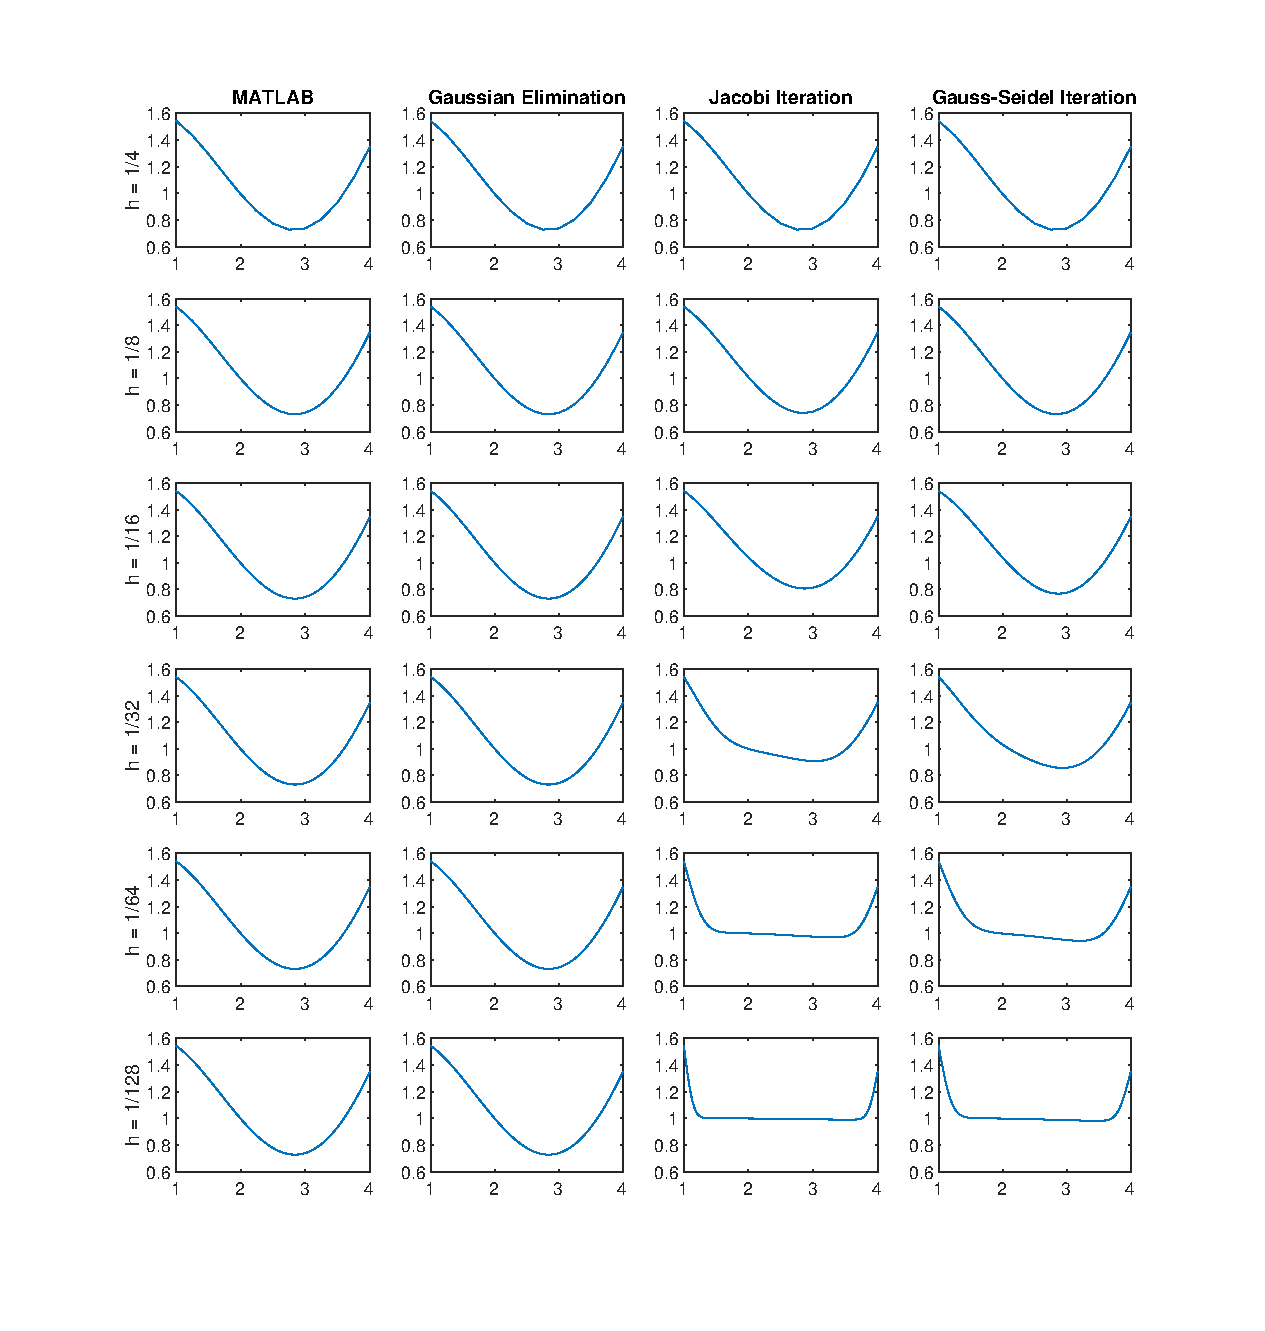
\includegraphics{plots.eps}
		\caption{Finite element approximations using different step sizes $h$ and different matrix equation solvers}
		\label{fig:plots}
	\end{figure}
	
	\question
	The maximum absolute errors on the nodes of the finite element approximations computed in Problem 9 are reported in Table \ref{table:p10}. See \verb*|p10_output.txt| for the commands entered in the command window to generate this data.
	\begin{table}[h]
		\centering
		\begin{tabular}{@{}lllll@{}}
			\toprule
			$h$ & \verb*|\| & \makecell{Gaussian \\ elim.} & Jacobi & Gauss-Seidel \\
			\midrule
			$\frac{1}{4}$ & 0.003971 & 0.003971 & 0.003957 & 0.003930 \\[.4em]
			$\frac{1}{8}$ & 0.000990 & 0.000990 & 0.012007 & 0.000632 \\[.4em]
			$\frac{1}{16}$ & 0.000248 & 0.000248 & 0.078263 & 0.044792 \\[.4em]
			$\frac{1}{32}$ & 0.000062 & 0.000062 & 0.186714 & 0.131855 \\[.4em]
			$\frac{1}{64}$ & 0.000016 & 0.000016 & 0.310389 & 0.227323 \\[.4em]
			$\frac{1}{128}$ & 0.000004 & 0.000004 & 0.420167 & 0.366232 \\[.4em]
			\bottomrule
		\end{tabular}
		\caption{Maximum absolute errors of numerical solutions at all nodes}
		\label{table:p10}
	\end{table}
	There are several observations that can be made about these results.
	\begin{itemize}
		\item The error using the MATLAB's \verb*|\| operator to solve the system decreases by a factor of roughly 4 each time $h$ decreases by a factor of 2. This is consistent with the second order convergence rate predicted theoretically.
		
		\item The error using Gaussian elimination is virtually the same as the error using \verb*|\| to solve the system. This makes sense, as Gaussian elimination solves the system directly, meaning that it's only error is due to floating-point round-off, and it should be equally as accurate as whatever method \verb*|\| uses.
		
		\item The error using the Jacobi and Gauss-Seidel iterative methods starts nearly the same as the error using \verb*|\| and Gaussian elimination, but as $h$ decreases, the error using the iterative methods actually \textit{increases}. This is not a defect of the finite element method, but a result of the slow convergence of the iterative methods.
		
		Empirically, I have observed that it takes more iterations for these methods to converge as $h$ decreases. For $h = \frac{1}{4}$, 200 iterations is sufficient to reach a tolerance of $10^{-5}$, but for smaller values of $h$, it is not. Thus, the reason for the increasing error is increasing error in the numerical solution of the linear system.
		
		Even if we set the number of iterations high enough to achieve a tolerance of $10^{-5}$, because the error in the finite element method is smaller than this for the smaller values of $h$, the iterative methods still fail to achieve the same level of error. Only if we set the tolerance much lower and the maximum number of iterations even higher do the iterative methods achieve accuracy comparable to \verb*|\| and Gaussian elimination for smaller values of $h$.
		
		\item The error using the Gauss-Seidel method increases more slowly than the Jacobi method, indicating that the Gauss-Seidel method has slightly faster convergence.
		
	\end{itemize}
	
	\bibliographystyle{plain}
	\bibliography{references.bib}
	
\end{document}